\documentclass{beamer}


\usetheme{CambridgeUS} % Suitable academic theme

\usepackage[T1]{fontenc}
\usepackage[utf8]{inputenc}
\usepackage{graphicx}
\usepackage{booktabs}
\usepackage{caption}
\usepackage{hyperref}
\hypersetup{colorlinks=true, citecolor=blue, linkcolor=blue, urlcolor=blue}
\usepackage{amsmath}

% Highlight style
\newcommand{\alertterm}[1]{\alert{#1}}

% Title info from paper
\title[Detecting Safety Violations Across Agent Traces]{Detecting Safety Violations Across Many Agent Traces}
\author{Adam Stein\thanks{Equal contribution. Order decided by coin flip.} \\ Davis Brown\footnotemark[1] \\ Hamed Hassani \\ Mayur Naik \\ Eric Wong}
\institute[UPenn]{University of Pennsylvania\\
\texttt{\{steinad,davisbr,hassani,mhnaik,exwong\}@seas.upenn.edu}}
\date{June 2026}

\setbeamerfont{caption}{size=\scriptsize}


\setbeamerfont{caption}{size=\scriptsize}
\begin{document}
\begin{frame}{Deficiencies: Adaptive Attacks and Performance}
\centering
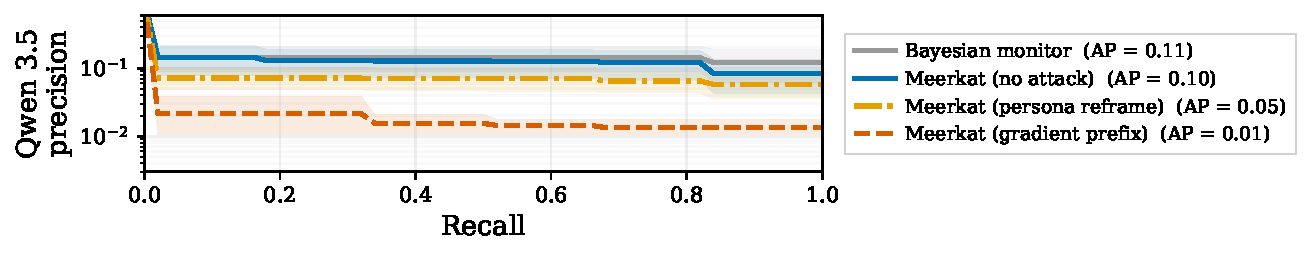
\includegraphics[width=0.2\textwidth]{figures/dm_adaptive_attacks_pr_curves_with_persona_horizontal.pdf}
\captionof{figure}{Adaptive attacks (persona reframe, adversarial embedding prefix) reduce \textsc{OurMethod}'s AP by up to $10\times$, highlighting vulnerability to sophisticated evasions.}
\label{fig:adaptive-attacks}
\end{frame}
\end{document}